\chapter{Container load balancing in cloud environment}
\label{mainidea}
\lhead{Chapter 2. \emph{Container load balancing in cloud environment}}

\section{Containers - Operating System-level Virtualization}

\subsection{Definition}

The technology of the operating system-level virtualization is composed of
different mecanisms to create isolated environments in the user-space.  Each of
those environment can gather one or several running applications and has access
to different resources. Those environment are commonly called containers from
the tool which popularized them: LXC (LinuX Containers). This technology is 

Operating system-level virtualization has been existing for a long time, it
appeared first in the BSD kernel (1998), where the technology is called
\textbf{Jails}.  Then, Sun developed Solaris (Sun UNIX operating system)
\textbf{zones} in 2005, the same year as the \textbf{OpenVZ} implementation for
the Linux kernel.

Containers are running over the same operating system as the host system, they
are sharing the same drivers, but all the processes contained in them are
limited by this same operating system. The memory consumption, the CPU usage,
the network and disk IO are monitored and managed by these container engines
sending the corresponding instructions to their respective kernel. 

This is a completely different approach to process isolation compare to
classical virtual machines. Where hypervisors and VM have been following the
paradigm where everything is virtualised, creating overhead and slower
performance, then we look at optimising by accessing hardware in order to
reduce binary translations and other slow operations. The main idea for
containers is, based on the host operating system, only the required
devices/features will be virtualised, and finally the level of performance is
close to native efficiency.

\begin{figure}
	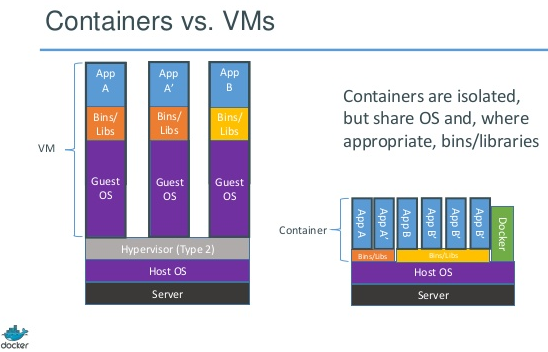
\includegraphics[width=\textwidth]{./Images/containers_vs_vms.png}
	\caption{Structural difference between containers and VMs}
\end{figure}

\subsection{Advantages}

Studying containers is not a random choice. They have been more and more
present in the industry these last years. Companies keep externalizing their
infrastructure, and the hosting of their services. The phenomena happens for
various reasons. A company infrastructure has to be robust, and available most
of the time. Nowadays, unavailability means important losses of money. As
hosting is a craft by itself, most of the companies do not have enough fund to
invest in a dedicated IT department, so they have to externalize thoses
processes.

The amount of resource providers, whether it is an application (Software as a
Service - SaaS), a platform (Platform as a Service - PaaS), or an
infrastructure (Infrastructure as a Service - IaaS), is increasing heavily,
because for the final users, it is cheaper than doing it themselves, and it is
easy to use, the internal mecanisms are abstracted.

Those providers have all the same problems: what is the best way to setup a
multi-tenant architecture which is secure enough and fast enough. "Containers"
is an answer to this issue. For example, the company \textbf{MongoLab} is hosting
thousands of MongoDB databases. Data is something critical for any company, so
\textbf{MongoLab} needs tot isolate each instance of MongoDB from each other.
We can assume that most of the databases they are hosting don't have a really high
traffic. Having a virtual machine for each of those instances is clearly something
oversized and would result on high provisionning overhead (duration of virtual
machine boot), storage overhead (1 full operating system per instance), etc.
This company is using containers because, it allows them to isolate the databases,
to provision them instantly, and the files required to run MongoDB are
only present once on their servers. (physical or virtual).

\subsection{Limits}

Containers are not able to live-migrate from one host to another with a
standard linux kernel yet. This feature is possible with a OpenVZ patched
kernel because thoses patches implement the checkpoint/restore operations for
the containers, but for a vanilla Linux kernel, it does not exist yet. Some
developers/hackers are trying to clean the code of OpenVZ and push the features
to the mainstream kernel with the \cite{websiteCRIU} project, but so far the
results are mostly drafty and unstable.

This main limit results in the difficulty to host stateful applications like a
database. It can be isolated in a container but we don't have the possibility
to move it without any downtime, the container has to be stop first then
restarted on another host. This is particularly blocking in the case of
production environment where every downtime leads to money loses for instance.

\subsection{Web Application}

As containerized stateful applications can not be cleanly load balanced among a
set of servers (a downtime is required), stateless web applications will be
targeted, as stated in the introduction of this work.

A Web application is an applicative server which uses the web standards to
communicate with clients. There are two main types of web services. The
websites, which are rendering HTML/JS/CSS web pages to users, and web services
defining an API and answering with standard data formats like XML or JSON. Both
of them are using HTTP as transfer protocol.

By the nature of HTTP, web applications are mostly stateless. Each resource
request is done using a new connection (except the case of reusing opened
connections). When a web application is stateful it is linked to the
application itself which is linking information to a local session or
connection.

These last 5 years, more and more of the web services have been written based
on some or all the principles of the REST method which declares as "best
practice" to create complete stateless applications. Additionaly, another
manifesto, the \cite{website12Factors} has become a standard set of good
practices for web development (website and web services)

The main advantage of stateless services is that they are able to scale
horizontaly easily: the first step is to spawn new instances of the service,
and then modify the routing table of a frontal reverse-proxy. As a result the
requests will be distributed among all the instances.

\subsection{Application balancing on the infrastructure}

When a web application has to be moved from one host to another, there should
be no unavailable time and the current requests have to stopped gracefuly. To
solve the first issue, the following walkthrough has to be followed:

\begin{enumerate}
	\item{Create a new instance of the application - Instanciate a new
	container of a web application}
	\item{Wait until the instance is available - TCP ping the application
	until a connection is established}
	\item{Change reverse proxy routing to route requests to the new
	container and not the old one}
	\item{Stop the old container to free its resources}
\end{enumerate}

To solve the second issue, it should be handle by the application itself. When
the system is querying the old container to stop. It actually sends a signal to
it.  In most systems (Systemd, Upstart at the system level, or Heroku and
Dotcloud at the PaaS level), SIGTERM is sent, then the application has some
time to shutdown. In the case where the application is still running a while
after receiving the signal, SIGKILL is sent to get rid of the process.

\subsection{Operation on containers}

\subsubsection{Load balancing}

The load balancing process consists in moving applications in order avoid having
over-loaded and under-loaded hosts.

\begin{figure}[h!]
	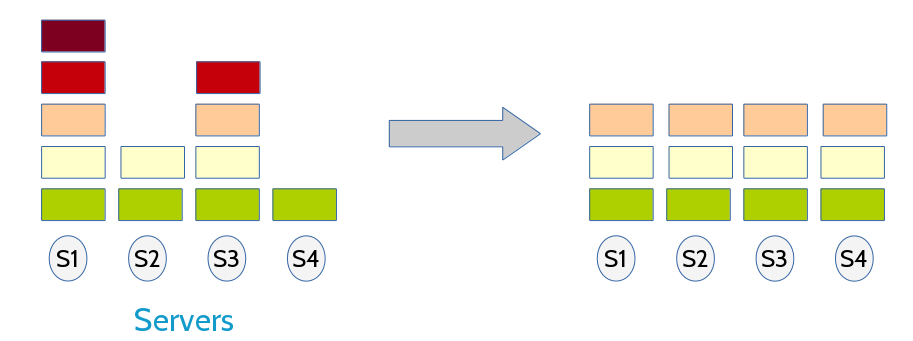
\includegraphics[width=\textwidth]{./Images/loadbalancing.png}
	\caption{Schema of a load balancing process}
\end{figure}

In most of the case, we can't really predict the evolution of the resource usage
of a service, this step has to be often to maintain a balance in an
infrastructure.  There are three potential outcome from this operation. The
first is, that the current number of hosts is sufficient, so the containers are
dispatched on them to get a balance of resource consumption. The second
possibility is that all the hosts are completely busy. In this case some new
servers should be provisionned. (Through a IaaS API, or more simply by sending
an email to the infrastructure manager who will have to deal with the
situation) The last case is when the hosts are not required anymore because
there the applications can be packed on less nodes that before. There are
different behavior which are possible in order to spare electricity and/or
money. If the hosts are VMs, they can be shutdown, if they are physical
servers, they could be suspended (If a mecanism like WakeOnLan is enabled to
wake them when they are required again) for example, these operationnal pieces
information are not in our scope.

\subsubsection{Resource Allocation}

Whan a new application has to start on the cluster, a container has to be
created.  At that step, it is required to find the best server to host this
newly spawned application

\begin{figure}[h!]
	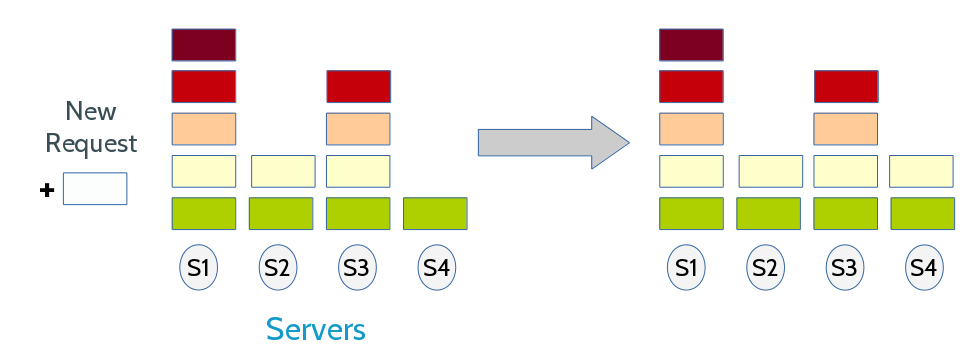
\includegraphics[width=\textwidth]{./Images/resourceallocation.png}
	\caption{Schema of a resource allocation process}
\end{figure}

For that step, it is required to find the most available server, because
deploying an application on a node which is already under an important load can
have repercussions on all the different containers hosted on it.
